\documentclass[a4paper, 12pt]{article}
%\usepackage[T1]{fontenc}
%\usepackage[latin1]{inputenc}
%\usepackage{concrete}
\usepackage{geometry}
\usepackage{multicol}
\geometry{top=2.5cm, bottom=3cm, left=3cm, right=2.5cm, nohead}
\title{Synthesizable Behavioral Design of a Video Coder}
\author{Vinicius Alexandre Kursancew}
\usepackage{graphicx}
\usepackage{subfig}
\usepackage{setspace}
\usepackage{hyperref}
\usepackage{lscape}
\usepackage{algorithmic}
\usepackage{algorithm}

\onehalfspacing

%\newcommand{\HRule}{\rule{\linewidth}{0.5mm}}

%\pagestyle{empty}
%\hyphenation{UCPel}
\begin{document}
UNIVERSIDADE FEDERAL DE PERNAMBUCO

GRADUA\c{C}\~{A}O EM ENGENHARIA DA COMPUTA\c{C}\~{A}O

CENTRO DE INFORM\'{A}TICA

\vspace{5cm}

\begin{center}
{\LARGE Synthesizable Behavioral Design of a Video Coder}
\vspace{1cm}
{\Large Vinicius Alexandre Kursancew}
\vspace{13cm}

RECIFE, BRAZIL

2009-06-22
\end{center}

\pagebreak
UNIVERSIDADE FEDERAL DE PERNAMBUCO

GRADUA\c{C}\~{A}O EM ENGENHARIA DA COMPUTA\c{C}\~{A}O

CENTRO DE INFORM\'{A}TICA

\vspace{5cm}
\begin{center}
{\large Vinicius Alexandre Kursancew}

\vspace{1cm}
{\LARGE Synthesizable Behavioral Design of a Video Coder}

\vspace{2cm}
This work was presented to the Centro de Informática of Universidade Federal de Pernambuco as a requirement to obtain the Computer Engineer Barchelor Degree.
\vspace{4cm}

\begin{tabular}{c}
\hline 
Vinicius Alexandre Kursancew \\
\end{tabular}
\vspace{3cm}

\begin{tabular}{c}
\hline 
Edna Natividade de Barros Silva (tutor) \\
\end{tabular}
\vspace{2cm}

RECIFE, BRAZIL

2009-06-22
\end{center}

\pagebreak


\section*{Acknowledegements}

I would like to thank my wife Renata, my daugter Nicole and my parents Alexandre and Renate for the all support and love they give me in every new onslaught that I'm involved, specially my father for his advises and for being my reference in ethics and morals.

I also thank all the professors from this University that mentored me in the course of my graduation. Their knowlege and advices was of great importance in the learning process.

\pagebreak

\begin{abstract}

This work describes the hardware implementation of a system capable of compression of digital picture sequences (digital video) into an MPEG2-video compatible data stream. The hardware is implemented using high level (behavioral) synthesis.  Just like RTL synthesis caused a revolution in the early 90s high-level synthesis is changing the pace that digital circuits are designed allowing the design houses to hit the short time-windows of the SoC industry. In the results of this work it will be possible to see that with just one high-level implementation several different hardware architectures could be generated and explored to pick the best result overall. One of this architectures was prototyped in an FPGA to validate the work.

Keywords: behavioral synthesis, video, video compression, mpeg, FPGA.

\end{abstract}


\pagebreak

\tableofcontents

\pagebreak

\listoffigures

\pagebreak

\listoftables

\pagebreak


\section*{Introduction}
\addcontentsline{toc}{section}{Introduction}

Complex IP Cores for the capture and compression of video in digital format such as H.264, MPEG-4 and MPEG-2\cite{mpeg2video} have an increasing demand in the consumer, military and medical applications. It is used in a diversity of digital cameras, Blurays and DVDs, Digital Television, industrial and military applications, among others. The implementation of streaming data processing hardware for these applications face the challenge of implementing and verifying the design before market window is gone, and as the market windows get narrower with time engineers are sometimes forced to release some design that might not be verifyed to the full extent because too much time was spent during implementation using the RTL synthesis methods developed two decades ago. 

Other than having to fit into tighter chronograms, designs are also getting more complex and integrated, and in the verification phase it keeps getting harder and harder to cover all test cases. A high level sythesis method would allow less effort to be directed to implementation, freeing resources for verification and quality assurance. Behavioral synthesis has grown significantly in the last years, from being considered "just academic research" into commercial grade products developed by the largest EDA vendors in the world, capable of cutting implementation efforts by up to ten times\cite{beh_grounds} and allowing much easier reuse of code.

Due to this promising context this works implements in hardware an MPEG2 video coder using a commercial grade behavioral synthesis tool.

In the remanescent sections the reader will find a short explanation of the behavioral synthesis process, then the general coding of picture sequences is detailed, followed by the actual behavioral implementation of the encoder. Finally, after results are presented, a conclusion seals the work by analyzing the results obtained. The reading of these sections imply basic knowledge of digital electronics and digital signal processing. If the reader needs embasement in those fields references \cite{digitalcircuits} and \cite{lyons_dsp} are recommended respectively.



\pagebreak

\section{A Short Introduction to Behavioral Synthesis}

	The rampant technological development that was experienced in the last forty years enabled the design and fabrication of higher and higher complexity electronics. One of the main actors in this technological progress are the automated design tools \cite{edahistory1}. Because of the high degree of miniaturization it became infeasible for an engineer to design and layout a complex integrated circuit (IC) "by hand".

	A process called synthesis was invented to relief the designer of some repetitive and error-prone tasks. Synthesis is the process of mapping some hardware decription into a lower-level equivalent, like converting a state machine description in the verilog language into registers and state transition logic.

	Other than simulation and verification tools, the first process to be automated was the layout of the ICs \cite{synthesisbook}, which were drawn in an almost artisanal way before the introduction of automatic placement and routing software during the late 60's. The next step was the logic synthesis, in which a technology independent set of boolean equations could be mapped to a specific technology, allowing the reuse of designs when the fabrication moved to a better process.

	During the 80's, when most of the largest current Electronic Design Automation (EDA) vendors went into business, a great effort was put into developing tools that allowed designers to specify the design in an architectural level. At this level the designer specifies registers, data paths and control and a tool would extract the required logic to implement that architecture. This process was called register transfer level (RTL) synthesis and for more than 20 years has been the standard entry point to digital IC design.

\begin{figure}[h]
\centering
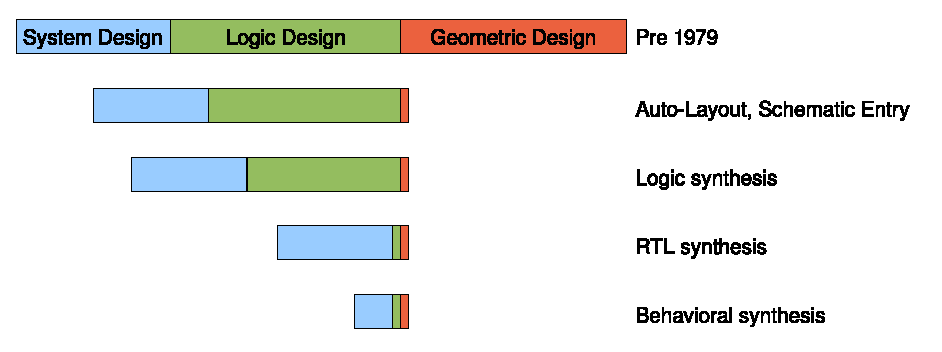
\includegraphics{figs/designeffort.eps}
\caption{Project speed-up for each design step improvement}
\label{fig:synthgains}
\end{figure}

	The most recent EDA tools can take a very high level input and go all the way down to silicon with little intervention from the designer. When the design behavior is specified as an algorithm (a list of sequential steps), containing no timing information, and that behavior is mapped in a RTL or logic description that process is called behavioral synthesis. Figure \ref{fig:synthgains} shows the average gain on development time for each of the processes listed above.


	Behavioral synthesis must perform three general tasks:
\begin{description}
\item[Scheduling:] assign each operation to specific a time slot, respecting the order of the operations;
\item[Resource allocation:] determine the type and number of resources used, like types of functional units (adders, comparators, etc) and registers; and
\item[Resource assignment:] instantiates the required functional units to execute the operations.
\end{description}

	This tasks will have to implement an architecture that not only is correct but also meets the design timing and silicon area requirements. In order to meet those requirements the behavioral synthesis tool provides the designer means of controlling the execution of those steps by specifying optimization and transformation directives, either globally or locally in each set of operations inside the code. 
	
	Below the constraints, optimizations and transformations mentioned through this work are explained:
\begin{description}
\item[Latency constraint:] the synthesis tool must schedule a certain block of operations in a specific number of clock cycles.
\item[Loop Unrolling:] when a loop is unrolled, instead of each iteration being executed sequentially the hardware is replicated and all (or a defined number) iterations execute in parallel. This of course will consume more area. Unrolling is not possible when inside the loop body a protocol transaction occurs, eg. a memory read.
\item[Loop Pipelining:] usually loop bodies are executed from the first statement to the last before starting the next iteration. If pipelining is defined the loop will start a new iteration at a specific cycle interval. This tends reduce latency without spending as much area resources as an unroll would.
\item[Array Flattening:] in a high level language the user does not instantiate memories or registers, the synthesis tools have to infer them. Usually arrays in the code are inferred to be memories, an array flattening directive would force the synthesis tool to infer registers from these arrays. Care must be taking when using this constraint on array with variable indexes because multiplexors are used to select the inputs and outputs of the registers, thus random accesses to a flattened array could cause the complexity of the design to explode.
\item[Data Path Optimization:] this is one of the most useful optimizations for data path oriented applications. It tells the synthesis tool to take a specific group of operations and implement a specific hardware block to execute that operations, that would otherwise be implemented using the standard parts from the technology library. When correctly applied data path optimization can save power, area and improve performance of the design.
\item[Chaining:] if chaining is enabled the synthesis tool will chain as much operations as it can in a single cycle, eg.: consider the expression $a + b + c$, with chaining disabled $(a+b)$ would be scheduled for one cycle, the result would be saved to a register and then in the next cycle the value of that register would be added with $c$. If chaining is enabled and the sum of the delay of two adders fit in a clock cycle, the expression would be calculated in one cycle.
\item[Aggressive Scheduling:] aggressive scheduling may be used when there is a branch in the code (usually an if-else or switch statement). The synthesis tool will try to implement the optimized branch as a data-path component and fit the result in a single clock cycle, whereas the regular behavior would be branching the state machine by placing a clock edge at the beginning of the conditional statement and merging it back where the code converges. This will reduce latency on some control-oriented constructs since it allows the number of control states to be reduced. 
\item[Synchronous Block:] the designer may specify a block of code where the operations are scheduled by him, manually. Each schedule cycle would be ended with a wait statement (in the case of SystemC).
\end{description}

	The tool of choice for behavioral synthesis was Forte Design Systems' Cynthesizer \cite{forteman} due to the availability of it's license to the writer. Cynthesizer's inputs consist of SystemC modules, synthesis scripts and a technology library, and it generates synthesizable RTL code code as output. Relevant competitor tools include Mentor Graphics's Catapult-C and Cadence's C-to-Silicon.

	In conjunction with Synplify Pro from Synplicity for logic synthesis and QuartusII from Altera for placement and routing the design that this work references was prototyped targeting a CycloneII FPGA device with 35.000 ALUTs. Section \ref{sec:tools} will present an overview of the flow that involves those tools.

\subsection{Synthesis Flow}
\label{sec:tools}

	This section will describe the process used to transform the behavioral design to the hardware implementation. This process involves several software from different vendors, the main one being the behavioral synthesis tool, Cynthesizer, from Forte Design Systems. The integration of the tools is all done through TCL scripting from Cynthesizer's project file. Figure \ref{fig:flow} gives an overview of the synthesis process.

\begin{figure}[h]
\centering
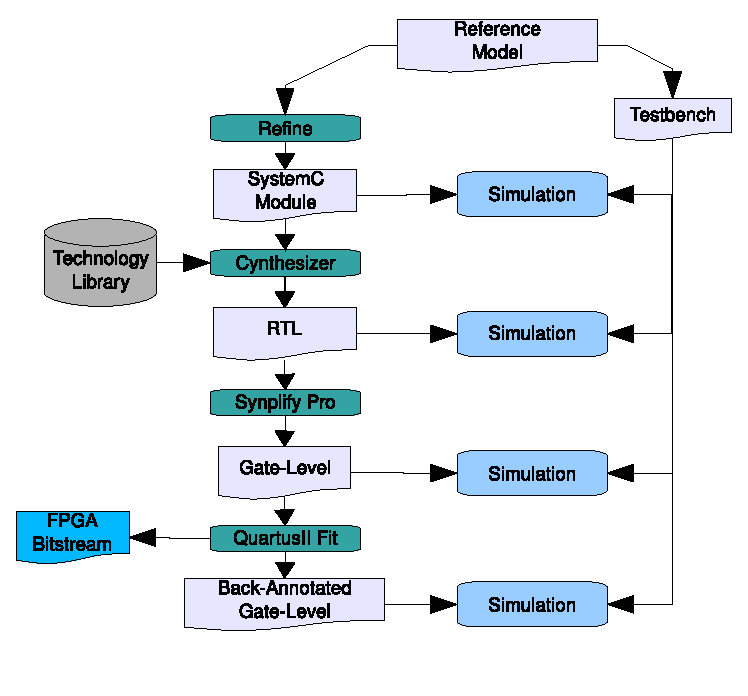
\includegraphics{figs/flow.eps}
\caption{Behavioral synthesis flow}
\label{fig:flow}
\end{figure}

The first step of the flow, which is to refine a SystemC module from a reference model, is optional, since the SystemC module can be written from scratch. But the test-bench still must be designed based on a reference model to ensure correctness.

After having the SystemC modules done the flow is as follows:
\begin{enumerate}
\item Synthesize the design to obtain RTL code
\item Optimize for throughput
\item Optimize for latency
\item Optimize for area
\item Run logic synthesis to obtain gate level description
\item Run placement and routing to extract parasitics and routing delays
\item Optimize to obtain timing closure
\end{enumerate}

Cynthesizer allows the user to explore a large area of the design space without too much effort. This is achieved through the placement of macros inside the SystemC code, and then, the macros are set according to the desired implementation options. This process of design space exploration is illustrated in figure \ref{fig:directive}. Each implementation option is then synthesized and the results are analyzed and the options that fall better into the design space are picked to go through logic synthesis.

\begin{figure}[h]
\centering
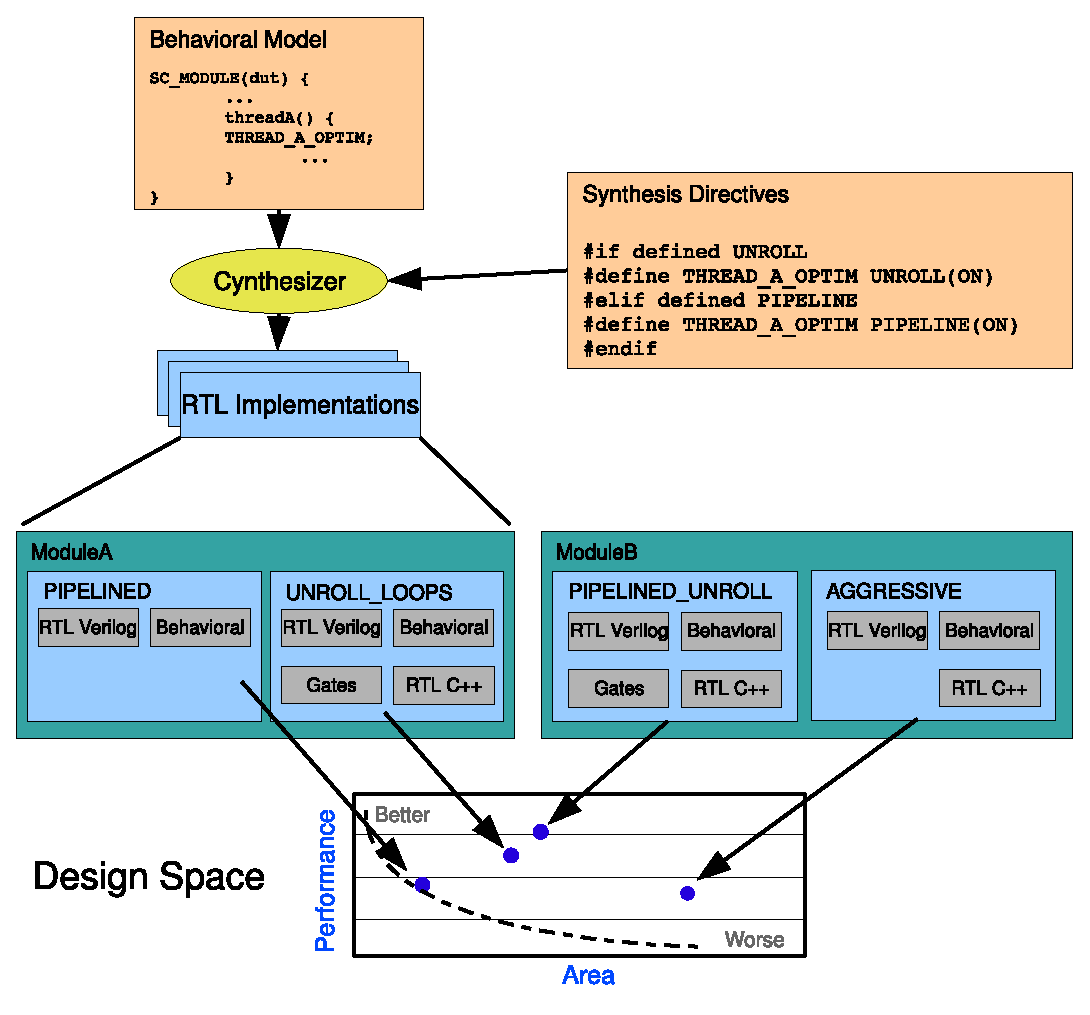
\includegraphics[width=15cm]{figs/cynthconfigs.eps}
\caption{Generation of multiple RTL implementations with a single high level design}
\label{fig:directive}
\end{figure}


\section{Coding of Moving Pictures}

	Transmission of moving pictures has always been known as a high bandwidth application. Due to this characteristic, since the beginning of analog television, techniques, such as chroma down-sampling and interlacing, have been used to reduce the bandwidth requirements to transmit video in a channel. As a result more channels could be allocated within the spectrum reserved for TV transmissions. Video compression has several other advantages, such as allowing longer play times for storage media, or if a given bandwidth is available it's possible to transmit a better-quality signal compared to an uncompressed one.

	Although compression has several benefits it also has some drawbacks and must be used wisely. The fundamental concept of compression is to remove redundancy of signals and only code the entropy contained in the data \cite{shannon}. However redundancy is the key to make data robust against errors, as a result a compressed signal is more error-prone than an uncompressed one. Compression also introduces latency in the signal, which is a great penalty for real-time systems. So as a general rule compression should be used only when needed, and not just for the sake of using it; and when used, parameters such as compression factor and algorithmic complexity must me chosen moderately, eg. if the restriction is the bandwidth do not compress further that needed to transmit the signal in that bandwidth.
	
	The advent of digital signal processing pushed the compression techniques to a new level allowing much higher compression ratios with very little quality compromise. Techniques used to compress digital video may be split into two main categories \cite{mpegbook}: Spatial Compression and Temporal Compression. Some compression is also achieved during pre-processing.

\subsection{Pre-processing}

	To be suitable for encoding data first must go through some pre-processing. The first step is to convert pixels to the correct colorspace. Colorspace is the way that a pixel is represented. The most usual representation is the (R,G,B) tuple that represents respectively the amout of red, green and blue that a pixel contains, but there are several other colorspaces such as CMYK, Hue-Saturation-Value, and Luma-Chroma. MPEG uses the Luma-Chroma format, specificaly the one known as Luma (Y), Chroma-blue (Cb) and Chroma-red (Cr). The Y component specifies the amout of brightness that a pixel has, and the Cb and Cr components are calculated as the difference from the brightness level to the level of the respective color component. There are several standards to convert from RGB to YCbCr, but the MPEG2 standard recommends the following:

$$ Y=\frac{0.299\times219.0}{255.0}R + \frac{0.587\times219.0}{255.0}G + \frac{0.114\times219.0}{255.0}B $$
\vspace{0.5cm}
$$ Cb = 0.564(B-Y)  = - \frac{0.16874\times224.0}{255.0}R - \frac{0.33126\times224.0}{255.0}G + \frac{0.5\times224.0}{255.0} + 128 $$
\vspace{0.5cm}
$$ Cr = 0.713(R-Y)  = \frac{0.50000\times224.0}{255.0}R - \frac{0.41869\times224.0}{255.0}G - \frac{0.08131\times224.0}{255.0} + 128 $$

\vspace{1cm}

	Another step performed before compression is the chroma sampling. The human eye is more sensitive to brightness information than to color. Therefore the sampling rate of the color information may be reduced without compromising the quality of the image. Usually luminance is sampled in the following ratios in respect to chrominance: 1/1, 2/1 or 4/1. MPEG suppot all of this formats, but usually chrominance is sub-sampled by a factor of four in comparison to luminance, this sample format called 4:2:0. As the MPEG processing is divided into 8x8 pixel blocks it's worth noticeing that for each four luminance that is transmmited one chrominance block of each type (Cb, Cr) is transmmited as pictured in figure \ref{fig:blocks}.

\begin{figure}[h]
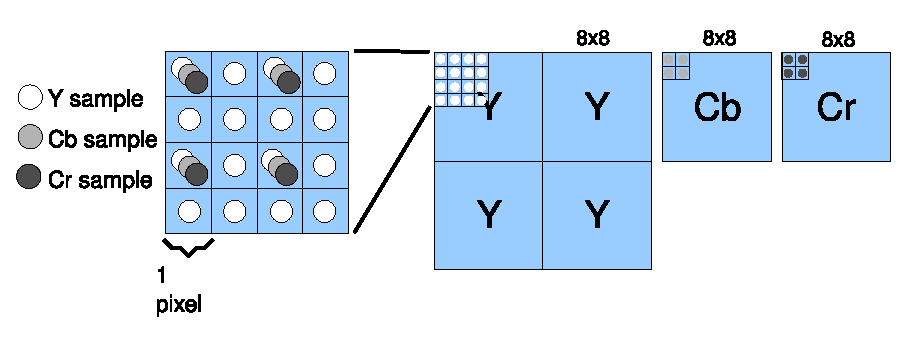
\includegraphics{figs/blocks.eps}
\caption{Luminance and chominance samples are sent in separate blocks}
\label{fig:blocks}
\end{figure}

	A step left as option, but recommended in case the source is noisy, is noise filtering. Noisy source material should be filtered because noise generates entropy, thus requires more bits to encode information that is not relevant to the picture.

\subsection{Spatial Compression}

	Spatial compression or intra-coded compression takes advantage of redundancy and perceptive features in a single frame. Gains in compression may be obtained because of large repetitive areas in the frame or because of the low sensitivity that the human eye has for noise in the high-frequency components of an image. Figure \ref{fig:spatialfreq} gives a feeling of what high and low frequencies mean in the spatial domain.

\begin{figure}[h]
\centering
\subfloat[]{ \label{fig:lowfreq} 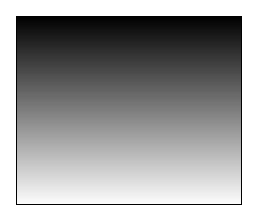
\includegraphics{figs/lowfreq.eps} }
\hspace{3cm}
\subfloat[]{ \label{fig:highfreq} 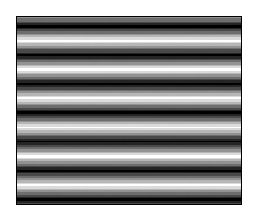
\includegraphics{figs/highfreq.eps} }
\caption{Images with (a) low, and (b) high spatial frequencies}
\label{fig:spatialfreq}
\end{figure}

	To achieve spatial compression the image is usually divided into blocks and transformed to the frequency (or more recently wavelet) domain, the most common way to do this is using the Discrete Cosine Transform (DCT), which is a special case of the Discrete Fourier Transform (DFT). The choice of the DCT over the DFT for video is because it makes it easier to remove redundancies and perform other processing, since all information that pertains to the high frequency components will be concentrated at the lower right of the transformed matrix and will, statistically, be very close to zero for real images \cite{gonzales}. Below is the regular formula for the two-dimensional DCT ( $ f[j,i] $ is the pixel at coorditates (j,i) ):

$$ F[u][v] = \alpha(u) \alpha(v) \sum_{i=0}^{i=N-1}{ \sum_{j=0}^{j=N-1}{f[j,i] \frac{\cos(2j+1)u\pi}{2N} \frac{\cos(2i+1)v\pi}{2N} }} $$

	Doing the DCT itself does not compress any data, the number of coefficients in the transformed matrix is the exact amount of pixels that the input contained. After transforming, the first manipulation done on the data to achieve compression is quantizing. To quantize means to represent some infinetely variable quantity by discrete stepped values. In case of video compression quantizing makes the steps between the range of the coefficient values larger, thus less bits are needed to represent the range. The process of discarding those bits cause an irreversible loss of informations. Thus, any compression technique, such as quantizing, that discards data is called lossy compression.
	
	Above it was mentioned that bits are discarded from coefficient data, but that process is not the same for all the components, higher frequency components are more quantized (have larger steps) than lower ones. That is because, to a certain level, they not perceptible to the human eye. Figure \ref{fig:quantizing}, which shows two images, (\ref{fig:quanthigh}) is the raw image and (\ref{fig:quantlow}) has bits discarded in the higher frequencies coefficients. The amount of bits discarded depends on the desired quality or bandwidth. In the case of this figure the raw image requires 111kB to store and the quantized requires only 9.7kB, this example gives a good measure of the compression gains that quantizing can achieve.

	Quantization also makes data redundant because the coefficients at the high-frequencies will have a great chance of becoming zero after quantized. Those zeroes can be coded efficently during a step called run-lengh coding, which is mentioned later in the text.

\begin{figure}[h]
\centering
\subfloat[Original]{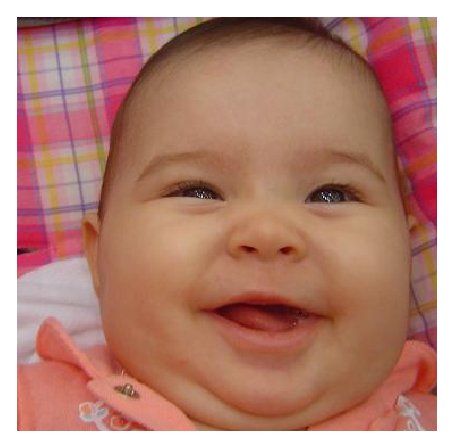
\includegraphics{figs/nic.eps} \label{fig:quanthigh}}
\subfloat[Quantized]{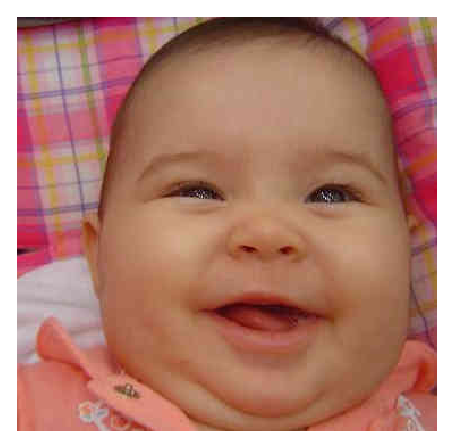
\includegraphics{figs/niclow.eps} \label{fig:quantlow}}
\caption{Two versions of the same image}
\label{fig:quantizing}
\end{figure}

	The next step is to take advantage of spatial redundancy: the DC coefficient of each block is coded differentially in respect to the previous, this will result in fewer bits to represent the data, for example: suppose two blocks of an image, A and B. A has a DC level of 120 and B a DC level of 131. If coded regularly 7 bits would be required for A and 8 for B. But if differential coding is used, A will use 7 bits but B can be coded as A+(+11) which requires only 5 bits. Substantial gain is obtained from this technique in scenes with low spatial frequency.

	Pictures that are coded using the techniques mentioned above are called intra-frames, and in MPEG jargon they are referenced as I-type frames. Intra frames are always the starting point of an entity called Group of Pictures in the MPEG standard. This entity 

\subsection{Temporal Compression}
	Subsequent frames in a movie sequence tend to have little changes.  This feature can be explored to reduce the amount of information that must be transmitted and send only the difference (also residual or prediction error) between the previous and current frames. This type of coding is called inter-coding, and a decoder that receives such type of frames must have a frame-buffer that is large enough to store the frames that may be referenced in the future. Theoretically any amount of inter-frames may be inserted between intra ones, but buffer size, random access capability and error propagation in the residual data limit this amount; in the case of MPEG2 video this value usually ranges from 0 to 12.
	
	Consumer devices, such as digital camcorders or cell phones may opt not to use temporal compression because doing so would raise the end-price of the product, rendering it economically infeasible. Another reason not to use inter-frames is in scenarios where fast random access to each frame is needed, eg. during video editing and production. If inter-frames are used, the access to a frame could require the decoding of several frames, introducing an annoying lag for the person handling the video.

\subsubsection{Motion Compensation}
	In common applications such as TV shows or movies the objects in the scene move in a continuous flow before a fixed camera, or the camera itself moves. Motion compensation is the technique that measures the motion of the objects in the frame so that difference between the current and previous frame can be made even smaller than of just taking the direct difference between each pixel. 

\begin{figure}[h]
\centering
\subfloat[Intra frame is coded]{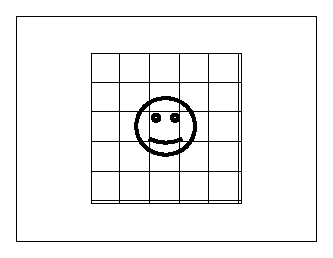
\includegraphics{figs/motiona.eps}}
\subfloat[Coding of inter-frame starts]{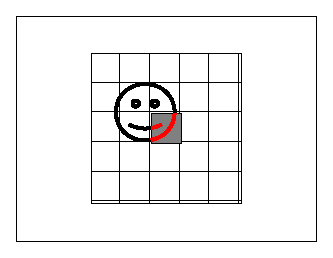
\includegraphics{figs/motionb.eps}}

\subfloat[Search for matching region]{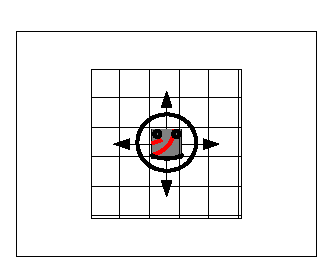
\includegraphics{figs/motionc.eps}}
\subfloat[Shift the region and subtract]{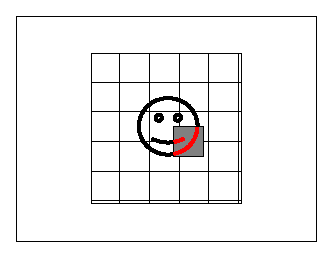
\includegraphics{figs/motiond.eps}}
\caption{Main steps of motion compensation}
\label{fig:motion}
\end{figure}

	Figure \ref{fig:motion} show the steps of motion compensation which are the following: (a) an intra-coded picture is sent as the reference and copied to a buffer. When the (b) next frame is to be coded, the coder will (c) perform a search in the stored picture for similar regions and extract motion vectors from the best match, which tells the direction and modulus of the movement. The objects from the previous frame are (d) shifted according to the vectors, this will cancel the motion, and at last the difference is calculated. This difference is called the prediction error, or residual. Both the motion vectors and the residual are transmitted instead of another intra-coded picture.

	The search step mentioned in the paragraph above is the most computation intensive. There are several approaches to search for a matching block in the previous picture: block matching, gradient, and phase correlation.

In block matching, a frame is split into a set of equal blocks. One block of the image is compared a pixel at a time against a block in the same region in the reference frame. If there is no motion, there is a high correlation between the two blocks. This is the most popular method due to it's simplicity and several approaches \cite{motionfss} \cite{motiontss} \cite{motionvlsi} \cite{motionhexagon} are suggested to overcome the computational complexity of doing a full search for the block, some of them are better for hardware and some for sowftware implementations.

The gradient method takes advantage of the relationship between spatial and temporal luminance gradients. When first adopted this technique seemed to be quite promising but it showed inefficient when exposed to irregular moving pictures such as scenes with explosions and flashes. In those cases the technique may confuse a spatial gradient with a different object in the reference frame.

Phase correlation is the most accurate and sophiticated motion estimation technique known. It's performed on the frequency domain, where object shifts are related to changes on phase of the transformed picture. After transforming both the reference and current pictures each phase component is then subtracted. The resulting difference is then transformed back to spatial domain and peaks will rise where there is motion between the two pictures.

\subsubsection{P and B Frame Types}
	
	Motion compensation may be used in a number of ways. MPEG-2 specifies two ways of coding inter-frames, one is called P-type frame and the other B-type frame.

	P-type frames can only reference material that is in the past with respect to the time line of the movie sequence. A rule that is applied in the MPEG-2 standard is that the P picture can only reference exactly the last frame, making it easier to implement a coder or decoder than in the case of the MPEG-4 standard that allows reference to many frames behind the current one, requiring much more picture memory.
	
	On the other hand B-type frames, which take this name from bidirectional motion compensation, can reference either past frames or frames that yet have to be decoded. For this reason a coding delay is introduced in the movie sequence and also the transmission order is modified to allow the referenced frames to be present on the decoder when the B-type frame arrives. Figure \ref{fig:reorder} show the correct order that frames are transmitted. An important rule for B-type frames is that they never reference each other or a loophole would be created on which would be transmitted first, as consequence of this they also do not have to be stored at the decoder for future use.

\begin{figure}[h]
\centering
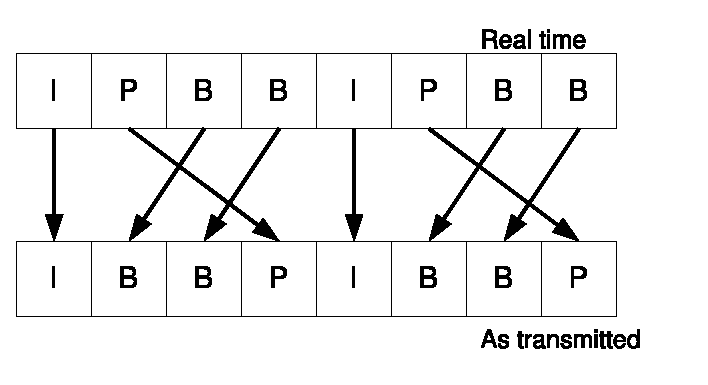
\includegraphics{figs/reorder.eps}
\caption{Ordering of pictures in an MPEG-2 stream}
\label{fig:reorder}
\end{figure}

\subsubsection{Removal of redundancy in data coding}

	The usual way that pixels are coded, usually using a fixed amount of bits per pixel factor, cause data redundancy. The last step on video coding is to remove as much redundancy as possible and coding only the entropy contained in the image. There are several methods for doing this, such as run-length coding, Huffman coding \cite{huffman}, Lempel-Ziv-Welch (LZW) coding\cite{lzw} and algebraic coding.

	These methods rely on statistics from real data to code the information in a way that most frequently used data is coded with less bits. More details on these techniques and involved theories are found on the references above and in .

\pagebreak

\section{Related Works}


This section will present two other works that are relevant to the analysis of this effort. The first one is an MPEG-4 video decoder developed by the Brazil-IP project and the other is an MP3 decoder developed using behavioral synthesis in UNICAMP.

\subsection{Behavioral SystemC Implementation of an MP3 Decoder}

Behavioral SystemC Implementation of an MP3 Decoder\cite{mp3beh} makes the comparison of the design of an MP3 audio decoder using behavioral synthesis against a hand-coded RTL implementation of the same specification. 

The design of this MP3 decoder is somewhat similar to the design proposed for the video encoder that is the subject of this text. This is due to the data flow oriented and pipelined nature of the MP3 decoding process, figure \ref{fig:mp3} shows that data flow.

\begin{figure}[h]
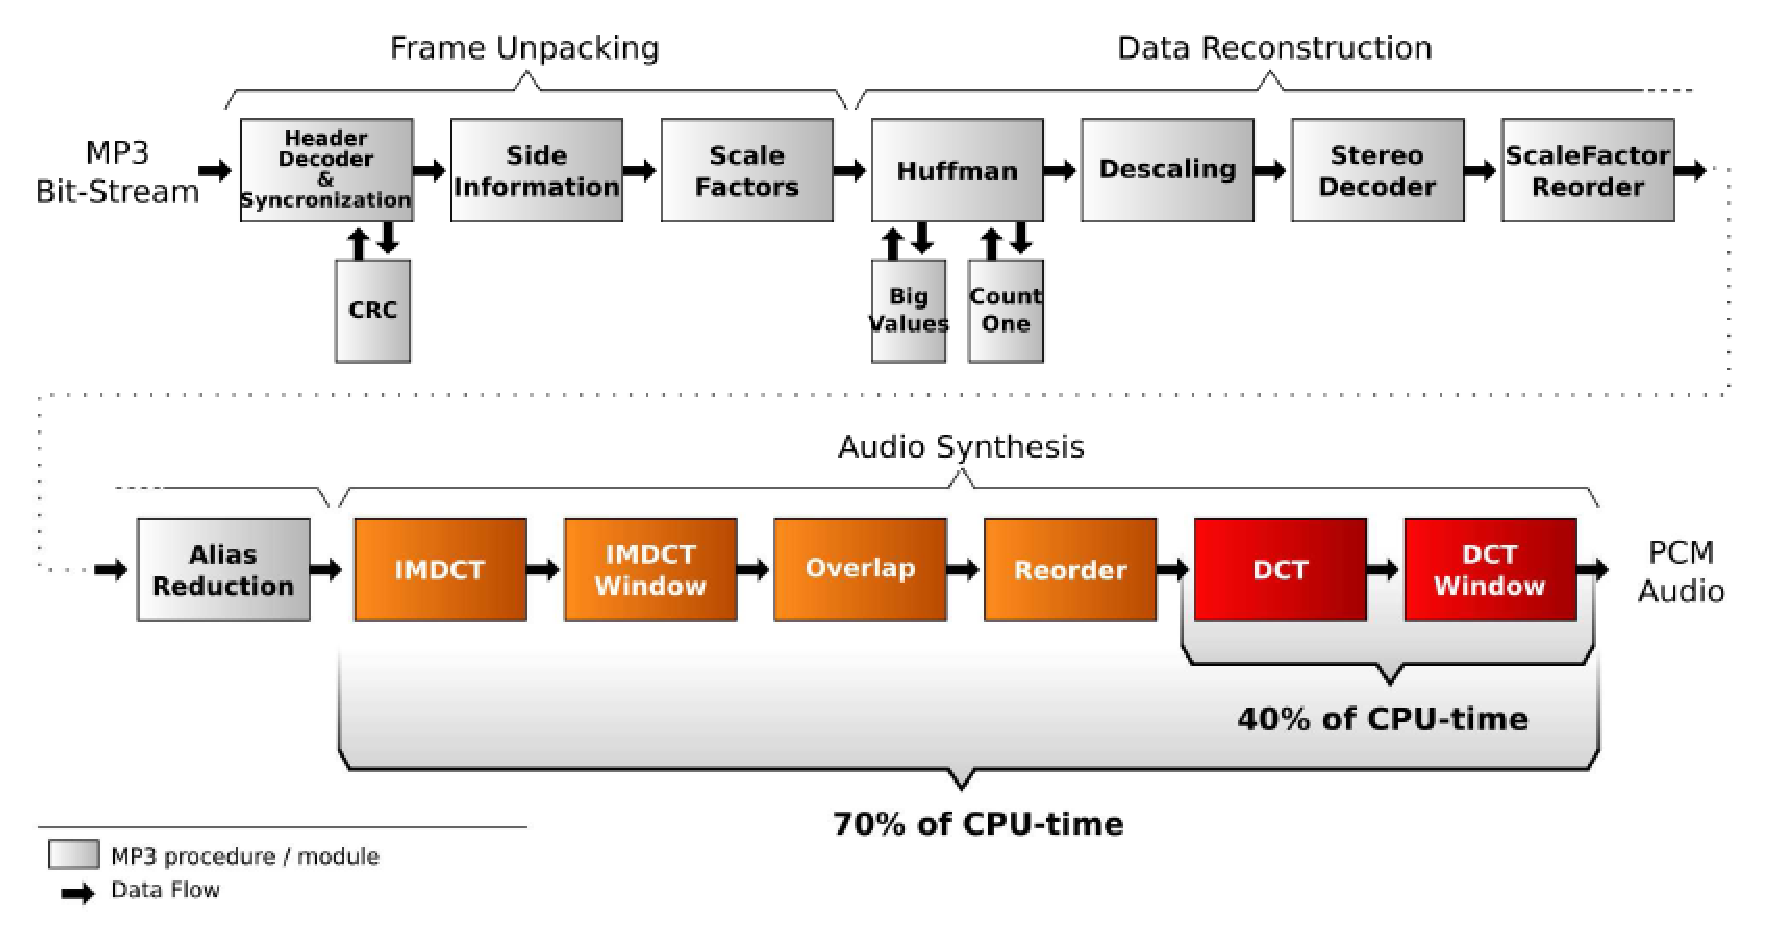
\includegraphics[width=15cm]{figs/mp3.eps}
\caption{Data flow pipeline of the MP3 decoder from \cite{mp3beh}}
\label{fig:mp3}
\end{figure}

The author from \cite{mp3beh} came to the same conclusion that the best code for software may result in a poor hardware implementation. Another point that the author mentions is that it was possible to test several different implementations withouth changing the code significantly. Some of the optimizations used in the MP3 encoder were loop unrolling, which improved latency 53\% while increasing area only 6\%, and pipelining, which improved latency by 42\% and increased 34\% in area.

As a conclusion the author makes the following comment:
"A single designer within a period of
3 months produced 14 design points using
the Forte Cynthesizer tool.
The same application, when designed in
SystemC RTL required 6 designers to
produce a single design point in one year"

\subsection{SystemC RTL Implementation of an MPEG-4 decoder}

The design of a decoder is quite similar to an encoder, one may even say that a decoder is a subset of an encoder since every encoder must also decode some of it's own encoded pictures for self-use. 

SystemC RTL Implementation of an MPEG-4 decoder \cite{brazilip} is a work that was prototyped in silicon using a total of about 48 thousand logic elements. The important information to extract from this design is the time it took to implement a single architecture using RTL: about two years with at least four people working on it. This information can later serve as a base comparison for the time it took to implement the MPEG2 encoder, which has at least twice the number of modules than a decoder does. Other figures such as frames per second and area are not so relevant because the picture size that the MPEG-4 decoder mentioned above can handle is 192x144 pixels, which is much smaller than the 720x576 resolution used in the encoder from this work.

\pagebreak

\section{A Synthesizable MPEG-2 Video Encoder}

	This section will present all the details of the design and implementation of a video coder which outputs a bit-stream compatible with the ITU H.262 (MPEG2 Video) standard \cite{mpeg2video}. First the top-level architecture will be presented followed by the verification strategies. Following that difficulties found during the implementation steps will be presented with the solutions found at each level: behavioral synthesis, logic synthesis and place and routing. 

	The effort on this encoder comes from an undergraduate research \cite{viship} that started in early 2007. At the time there was availability to use a high synthesis tool for a research project. Video coding was chosen because its algorithms \cite{chendct} \cite{motion}  are data path oriented, this makes them very good to be implemented using behavioral synthesis because many different behavioral transformations can be applied giving a large design space to be explored.

	During the initial phase of the project a hardware design process called ipProcess \cite{ipprocess} was used to map the requirements into the design shown in section \ref{partitioning}.

\subsection{Design Requirements}

	Before the start of the project a few basic requirements were settled to limit the scope of the project, they were chosen based on the applicability to consumer electronics, for example, DVD players. The requirements are the following:
\begin{description}
\item[Resolution:] The chosen resolution was 720x576, which is the standard resolution for digital television and DVDs.
\item[Scan order:] Progressive scan order was chosen instead of interlaced. Interlaced scan is a legacy from analog TV, in which all odd lines are send before the even ones. Digitally coding and compressing interlaced pictures is supported on the MPEG-2 standard but is not efficient and should not be used when the original source is available in progressive scan order. Coding of interlaced sequences is still possible if a de-interlace filter is applied before coding.
\item[Frame Rate:] 24 frames per second were chosen because it is the recommended minimum for standard definition movies.
\end{description}

\subsection{Top Level Design Partitioning}
\label{partitioning}

\begin{figure}[h]
\centering
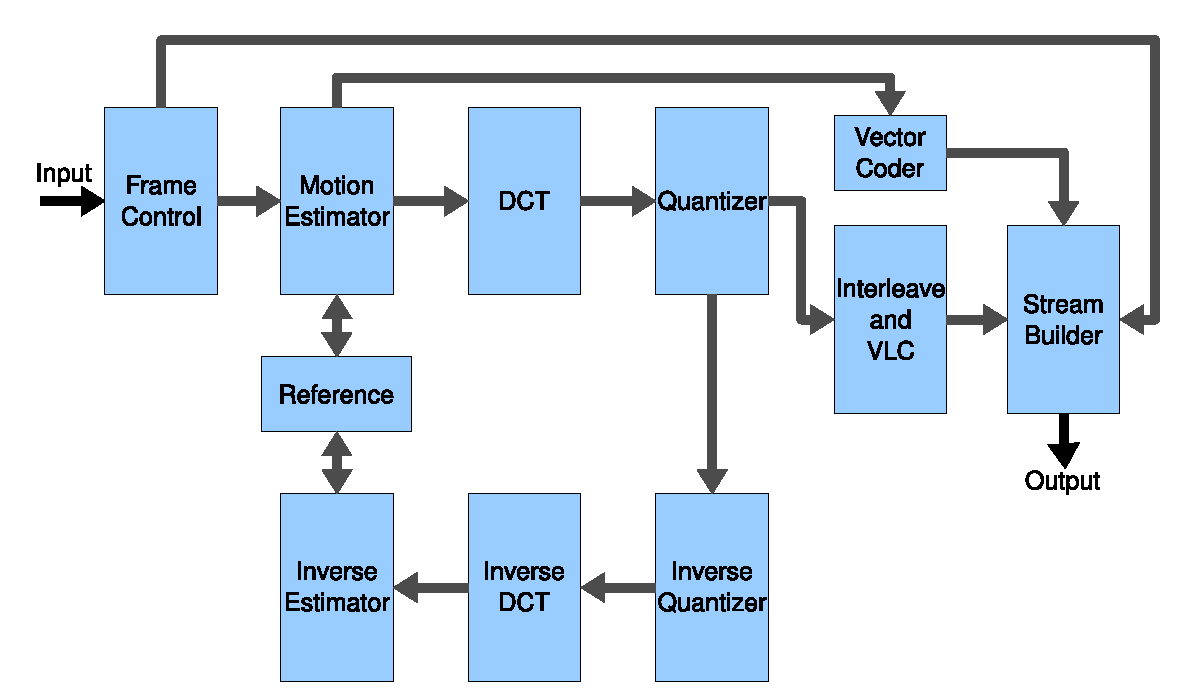
\includegraphics[width=15cm]{figs/top.eps}
\caption{Top level partitioning for the MPEG-2 Video encoder.}
\label{fig:top}
\end{figure}
	The first step for a successful synthesizable behavioral design is to properly identify design partitions, which can be implemented as independent threads.

	The encoding task can be broken down into several independent modules, in the case of this encoder ten modules: Frame Control, Motion Estimator, DCT, Quantizer, Interleaver and Variable Length Coder, Motion Vector Coder, Stream Builder, Inverse Quantizer, Inverse DCT, Inverse Estimator and Reference. The modules are connected in a pipelined fashion, as seen in figure \ref{fig:top}, and each module can process one 8x8 pixels block at a time.
	
	It is relevant to notice the reverse path of the encoding process, where the frame is decoded to generate a correct reference for the motion estimation process. If the original picture would be used the decoded picture would have crude errors because the decoder only has access to the frame that was coded and quantized, thus had information thrown out.
	
	In the sub-sections below, each module will have its functionality explained and also comments will be made about possible optimizations applied to the module.

\subsubsection{Frame Control}

	The Frame Control module is responsible for acquiring the input pixels and packing them into 8x8 blocks and deciding which type of frame the current frame is: inter or intra. It has a more control-oriented nature and the only directives used were latency constraints. 

	This module is also replaceable depending on the type of input that will be given to the coder: a camera, memory, a storage device, etc.

\subsubsection{Motion Estimator}
	The Motion Estimator tries to find in a past reference frame some content that is similar to the current block being processed. The algorithm used is an adaptation of the simple three-step search presented in \cite{motiontss}. In this algorithm first a crude search is performed, and then the algorithm makes a finer search in the region with the lowest sum of abslute differences. This algorithm's main flaw is the high succeptability to fall into a local minima in the first step, causing more data than necessarry to be coded as prediction error. Algorithm \ref{motionalg} describes the computation steps performed in this module. It tries to find the matching block with the lowest mean absolute difference (MAD) within a defined window. 

\begin{algorithm}[H]
\caption{Motion estimation algorithm for one macro-block (16x16 pixels)}
\label{motionalg}
\begin{algorithmic}[1]
\STATE Let $f(x,y)$ be the current frame and $r(x,y)$ the reference frame.
\STATE Let $c$ be the macro-block subject to the search, with top-left coordinates at $x_s$ and $y_s$ in $f(x,y)$
\STATE Let $mad(x,y)$ be a function that returns the MAD of $c$ and the block with top-left coordinates at $r(x,y)$
\STATE Let there be three set of touples $DV[1..3]$ containing relative values of displacement vectors for each step of the search.
\STATE Initialize the motion vector $\vec{v} \leftarrow (0,0)$
\STATE $MAD_{min} \leftarrow mad(sx,sy)$
\STATE $x_{min} \leftarrow x_s$
\STATE $y_{min} \leftarrow y_s$
\FOR{$k=1$ to $3$}
\STATE $x_{center} \leftarrow x_{min}$
\STATE $y_{center} \leftarrow y_{min}$
\FOR{$i=1$ to $length(DV[k])$}
\STATE $x_p \leftarrow x_{center} + DV_{x}[k][i]$ (truncate if $x_p$ is out of the frame size)
\STATE $y_p \leftarrow y_{center} + DV_{y}[k][i]$ (truncate if $y_p$ is out of the frame size)
\STATE $MAD \leftarrow mad(x_p, y_p)$
\IF {$MAD < MAD_{min}$}
\STATE $x_{min} \leftarrow x_p$
\STATE $y_{min} \leftarrow y_p$
\STATE $\vec{v} \leftarrow (x_p - x_s, y_p - y_s)$
\ENDIF
\ENDFOR
\ENDFOR
\RETURN $\vec{v}$, the motion vector and $MAD_{min}$, the error
\end{algorithmic}
\end{algorithm}
	
	This task is protocol-intensive since during the $mad(x,y)$ function it must fetch many pixels from the reference frame, which is contained in an external memory. Effort should be made towards reducing the latency between each read and maximizing throughput of each transaction with the external bus. One approach to this may be pipelining the module, so that while pixels are being processed the next ones needed are being fetched.

\subsubsection{DCT}
	Each coded block of the frame is transmitted in the frequency domain. The Discrete Cosine Transform is used in the MPEG2 standard to accomplish this task.
		The DCT of this design is based on the Chen Fast DCT algorithm \cite{chendct}, generalized to the two dimensional case, where first the DCT is calculated for each column and then on the resulting matrix each row is also transformed. The arithimetic is all fixed point and 12 bits are used to preserve acuracy. Figure \ref{fig:dctbutterfly} shows a data-path diagram for the operation performed on each column (or row), the cossing operations on this diagram receive the acronym of butterflys due to the resemblance with the insect of that name. If the flow is performed from left to right the operation is the forward transform, and if done from the opposite it's the inverse DCT. White circles represent adders, and squares multiplications with constants.

\begin{figure}[h]
\centering
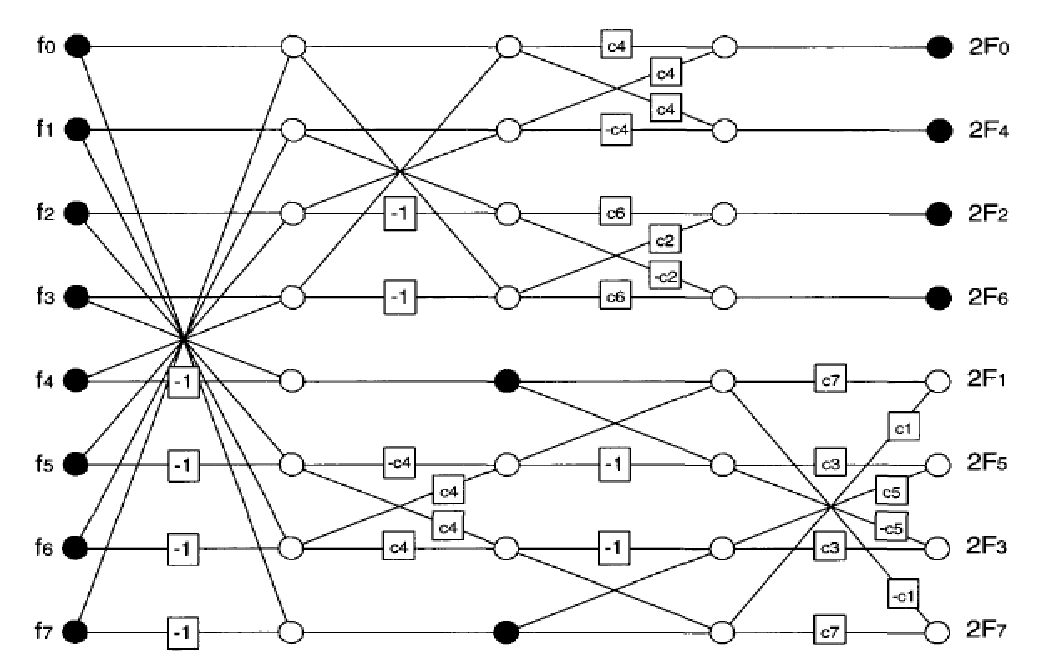
\includegraphics[width=15cm]{figs/butterfly.eps}
\caption{Fast DCT data flow}
\label{fig:dctbutterfly}
\end{figure}

	This module is highly data path oriented and is subject to many optimizations: internal arrays are flattened, data path can be optimized and the execution loop may be pipelined.

\subsubsection{Quantizer}
	The Quantizer will take as input a set of coefficients from the DCT module and discard bits according to the relevance of that frequency component to the human vision. The quantization method can either be constant, linear or non-linear. In the case of this encoder the constant method was chosen. Using a variable quantization method would imply the implementation of a bit-rate control mechanism, which was excluded to simplify the design.
	
	This task is highly data path oriented and requires access to a constant table, which is flattened, to allow the use of loop unrolling.

\subsubsection{Interleave and VLC}
	As a final step in the encoding process the data is compressed using variable length coding (VLC) with zero run length coding for frequency components that are not present in the block. To have better results for the zero run length coding the data is first interleaved (reordered) in a way that it's more probable that a large run of zeros will occur. After that the VLC is performed. 
	
	This is a control intensive task and benefits from the aggressive scheduling of control branches.

\subsubsection{Motion Vector Coder}
	The motion vectors that are calculated by the motion estimator need to be coded using variable length coding, just like the frequency components of the blocks. Another processing that is done in this module is to code only the difference between successive vectors, this saves more bits since motion in pictures tend to follow an ordered flow. This module is control oriented and benefits from aggressive scheduling of control branches.

\subsubsection{Stream Builder}
	The MPEG2 format has it's headers and specifies a specific order which motion vectors and block data must appear in the stream. This module is responsible for placing the headers and multiplexing the data coming from the modules in the correct order. 
	
	It's a pure control module, with a few branches, which receives as input data from the Frame Control, Interleaver and VLC, and Motion Vector Coder modules.

\subsubsection{Inverse Path Modules}
	Motion Estimator, DCT and Quantizer modules each have their inverse counterpart with the purpose of decoding and rebuilding the coded blocks to form the reference frame for the Motion Estimator. This has to be done to keep information coded consistent with the information that will be available to the decoder as mentioned above. 
	
	The directives for each inverse module are the same as their coding counterpart.

\subsubsection{Reference}
	The Reference module stores two frames, the current reference and the next reference. The sole purpose of this module is to manage the access to the memory that contains the reference data, since two modules need access to it: the motion estimator for reading and its inverse for reading/writing.

\subsubsection{Interfaces Between the Modules}

	The modules in this design must somehow interface to each other. On a regular RTL design the interfaces could be determined dependant on timing, since the designer knows exactly when some data will be available to be processed. On behavioral designs the latency of the operations is not fixed, and depending on the synthesis directives and effort a different RTL architecture, in which timing parameters do not match, may be generated. Said that an approach for this is implementing a four-state protocol, with data ready and data valid signals, as detailed on the waveforms of figure \ref{fig:protocol}.
The waveform shows a case where data is read before it's written and next a case where data is written before it's read. The triangles on the data signal represent the storage of data by the reader. 
\begin{figure}[h]
\centering
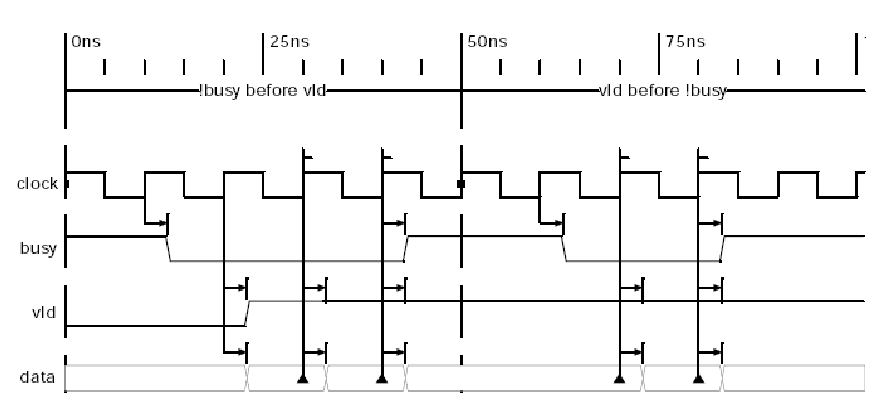
\includegraphics[width=15cm]{figs/p2pprotocol.eps}
\caption{Four state protocol waveform. }
\label{fig:protocol}
\end{figure}

	Implementing this protocol for each module interface introduces a great overhead and a potential source of bugs, since each interface would be hand coded. To make the task of implementing that protocol easier the designer may use modular interfaces that are templatable. Modular interfaces is the concept of encapsulating the interface code in such a way that when the designer wants to use it all he needs to do is to instantiate a input or output port from that interface and calling the respective functions from the interface API, for example, if the user wants to write to a port called OUT he would just call OUT.put(x) and the put function would implement the protocol semantics, that is for any protocol. Other than encapsulating the communication code this approach allows experimenting with different protocols just by replacing the type of the port, providing it maintains API compatibility. 

	The interfaces used on this design were taken from Cynthesizer's interface library, called cynw\_p2p. The user may transmit any data type, including arrays and entire structures. Using verified interface IP saved precious time that would be wasted with protocol implementation and debugging. The code snippet on figure \ref{fig:protocolcode} shows the usage of this interface library and it gives an overview of some of the advantages of using modular interfaces.

\begin{singlespace}
\begin{figure}[h!]
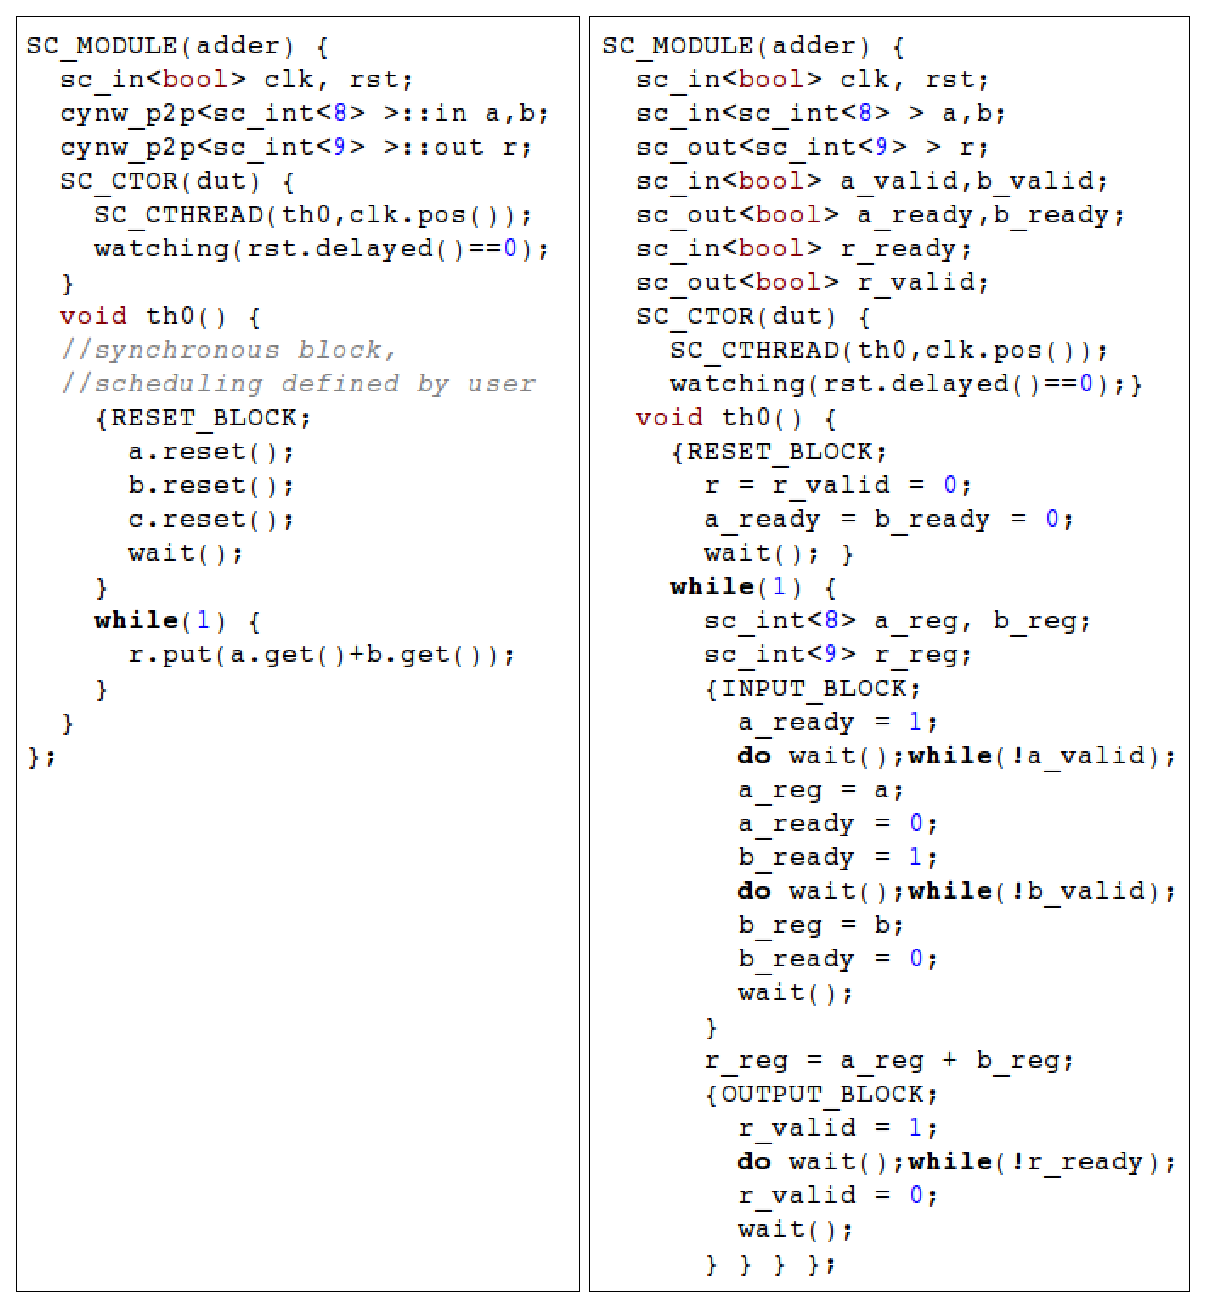
\includegraphics[width=15cm]{figs/p2pcode.eps}
%\begin{multicols}{2}
%
%\begin{verbatim}
%SC_MODULE(adder) {
%  sc_in<bool> clk, rst;
%  cynw_p2p<sc_int<8> >::in a,b;
%  cynw_p2p<sc_int<9> >::out r;
%  SC_CTOR(dut) {
%    SC_CTHREAD(th0,clk.pos());
%    watching(rst.delayed()==0);
%  }
%  void th0() {
%  //synchronous block, 
%  //scheduling defined by user
%    {RESET_BLOCK; 
%      a.reset();
%      b.reset();
%      c.reset();
%      wait();
%    }
%    while(1) {
%      r.put(a.get()+b.get());
%    }
%  }
%};
%\end{verbatim}
%
%\vspace{9cm}
%
%\begin{verbatim}
%SC_MODULE(adder) {
%  sc_in<bool> clk, rst;
%  sc_in<sc_int<8> > a,b;
%  sc_out<sc_int<9> > r;
%  sc_in<bool> a_valid,b_valid,r_ready;
%  sc_out<bool> a_ready,b_ready,r_valid;
%  SC_CTOR(dut) {
%    SC_CTHREAD(th0,clk.pos());
%    watching(rst.delayed()==0); }
%  void th0() {
%    {RESET_BLOCK;
%      r = r_valid = 0;
%      a_ready = b_ready = 0;
%      wait(); }
%    while(1) {
%      sc_int<8> a_reg, b_reg;
%      sc_int<9> r_reg;
%      {INPUT_BLOCK;
%        a_ready = 1;
%        do wait(); while(!a_valid);
%        a_reg = a;
%        a_ready = 0;
%        b_ready = 1;
%        do wait(); while(!b_valid);
%        b_reg = b;
%        b_ready = 0;
%        wait();
%      }
%      r_reg = a_reg + b_reg;
%      {OUTPUT_BLOCK;
%        r_valid = 1;
%        do wait(); while(!r_ready);
%        r_valid = 0;
%        wait();
%      }
%    }
%  }
%};
%\end{verbatim}
%\end{multicols}
\caption{Comparison code using modular interfaces versus regular protocol blocks.}
\label{fig:protocolcode}
\end{figure}
\end{singlespace}

\subsection{Verification of the Design}

Just like any hardware design the MPEG2 encoder presented on this text was verified to ensure correctness of it's functionality. There are two basic types of verification for hardware design: formal equivalence checking, and functional verification. In formal equivalence checking the design is proven to be formally equivalent to a specification at a higher level, that is taken as correct. Functional verification relies on driving the design with known stimuli and observing it's behavior to check if it responds as expected.

Function verification was chosen to be used in this design because it's more practical and the design environment provided by the behavioral synthesis tool has much better support for it than formal equivalence checking.

One of the advantages of using functional verification in behavioral designs is because the design itself may be refined from the reference model, which is the case of the encoder presented here. First a reference model was designed and checked for correctness with an MPEG2 stream analyzer from the MPEG test group \cite{mpeg2dec}, after that a set of golden files (files which are taken as being the correct output for a given input) was generated for each module. After that the reference model was refined to serve as input for the synthesis tool.

\subsubsection{Verification Environment}

The environment described in this section is suggested by the design methodology guide from Cynthesizer. It comprises of a test bench, which generates and read stimuli and a design under verification (DUV). Figure \ref{fig:tbduv} shows the actual setup if this verification scheme, notice that a DUV may have more than one module, and the modules need not to be running at the same abstraction level. 

\begin{figure}[h]
\centering
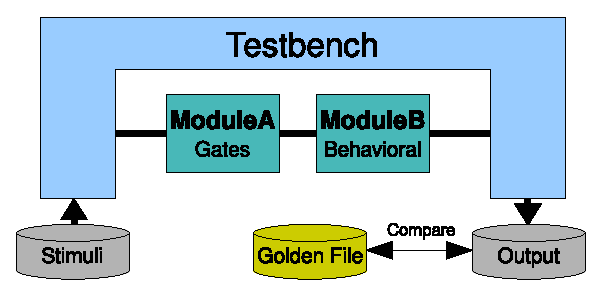
\includegraphics{figs/testbench.eps}
\caption{Setup for functional verification}
\label{fig:tbduv}
\end{figure}

With the setup that was introduced above the design can be verified at any level of abstraction or synthesis configuration. Five different levels of abstraction were used:

\begin{description}
\item[Behavioral-level pin-acurate simulation:] In behavioral simulation the design is simulated in a SystemC environment, and all the statements, except for protocol blocks, are untimed. This is the baseline by which simulations of synthesized modules are compared. For this case a pin-acurate port interface was used but transaction-level ports can also be used, in this case  even the protocols would be untimed.

\item[C++ RTL simulation:] This is the first output from the synthesis tool. It also simulates at a SystemC environment but all the design is timed according to the schedule defined by the synthesis tool. Mismatches at this level may occur because of bugs in the synthesis tool or because of failure to comply with the design guidelines specified by the synthesis tool vendor.

\item[Verilog RTL simulation:] This level is just like the C++ RTL simulation, but the design is transformed into verilog, which is the input to most RTL synthesis tools. Some design problems may be caught at this level, like missing a reset statement in the SystemC design.

\item[Gate-level simulation:] After the behavioral synthesis tool is done the design still needs to pass RTL synthesis and mapping. This level of abstraction simulates the design plus inserts the propagation delay of logic gates. Simulations tend to fail at this level if the synthesis tools constraints were too tight.

\item[Back-annotated gate-level simulation:] This level includes even more information on the final implementation of the design, like routing delays. If a design passes at this level it's highly probable that it'll work.
\end{description}


\subsection{Design Difficulties}

This section will present some challenges that were faced during the design of the encoder. Also, when it's possible, the approach to avoid the problem is presented. Since logic synthesis did not present any relevant difficulties during it's flow it's not commented in the sectionns below.

\subsubsection{Behavioral Synthesis}

The first problem encountered during the behavioral synthesis is that not every behavioral code will give out a good hardware implementation, sometimes the best alternative in software may not synthesize at all (even if it only uses supported constructs) because the complexity of the hardware cannot be handled by the available hardware (CPU/memory). Some characteristics of optimized software that don't synthesize into good hardware are:

\begin{itemize}
\item Usage of dynamic memory: synthesis tools cannot free or allocate memory, synthesis is not even possible in this case.
\item Using RAM look-up tables with pre-calculated values: usually in hardware it's much faster and cheaper to place the logic to do the calculations on the fly.
\item Branching to skip calculations: branching makes hardware much harder to schedule. Branching will either reduce performance or increase area, depending if aggressive scheduling is turned on or off.
\end{itemize}

A lot of valuable knowledge on this kind of details was obtained on a first synthesis try with an encoding software from the MPEG test group. 
It was perceived that too much effort would be required to refine the code from the software from the MPEG test group, so it was decided to redesign and implement the encoder from-scratch, with behavioral synthesis in mind. Other than acquiring knowledge this software served as a comparison to implement the reference model for the encoder presented on this work. Some of the main points on problems during behavioral synthesis are outlined in the following paragraphs. 

The behavioral synthesis problems will be split into four categories:
\begin{description}
\item[Unschedulable design:] an unschedulable design is a design that the sysntesis tool finds some operation that is impossible to schedule due to an implementation mistake or tight constraint. Figure \ref{fig:schedfail} shows a data path that fails to schedule within a defined clock period of 20ns.
\item[Unexpected area growth:] it's when the area of the synthesized design ends up being much larger than expected, usually due to a bad usage of some optimization or construct.
\item[Unexpected complexity growth:] before starting the whole synthesis process the synthesis tool builds an internal representation of the design. In some cases this representation becomes too complex the synthesis may take long to finish (days or weeks) or simply fail due to lack of memory, and the design will most probably not pass logic synthesis.
\item[RTL simulation mismatch:] this problem is characterized by a difference in behavior between the high-level specification and the generated RTl. Many times it's because of designer mistakes, like missing reset statements, but some times it's because of tool peculiarities which may turn to be very hard to fix.
\end{description}

\begin{figure}
\centering
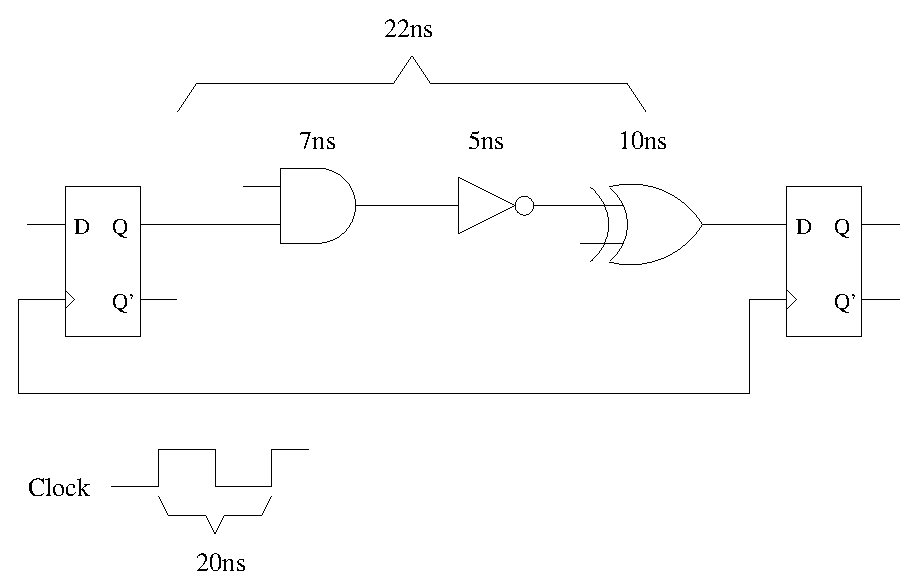
\includegraphics{figs/schedfail.eps}
\caption{A datapath failing to fit the clock scheduling.}
\label{fig:schedfail}
\end{figure}

One of the earliest synthesis tries showed that excessive branching, specially inside non-constant loops (loops that the iteration count is not known) will generate poor hardware. This is because the synthesis tool will implement the exact same behavior in the hardware, and branches are implemented either with muxes or FSM branching and merging. If the mux option is selected for synthesis then the design may fail scheduling because the mux path delays may not fit in the clock period, and if the state-machine branching option is used for synthesis then the synthesis tool may not be able to code the FSM in reasonable time. The solution for this is to write code in such a way that the flow is somewhat consistent for all inputs and move control structures out of loops.

The next point is about array flattening. As mentioned before, flattening arrays will cause them to be implemented as registers and not memories. All the access logic to those register must then be implemented with multiplexors. Improperly flattening arrays will cause area to grow in an unexpected way, some cases were observed that more than 60\% of the FPGA logic was used for muxing, this design of course would be doomed to fail placement and routing. The main cause of bad hardware due to flattening is non-constant access to indexes of the arrays. Figure \ref{fig:flatten} shows an example where flattening is used improperly.

\begin{figure}[h]
\centering
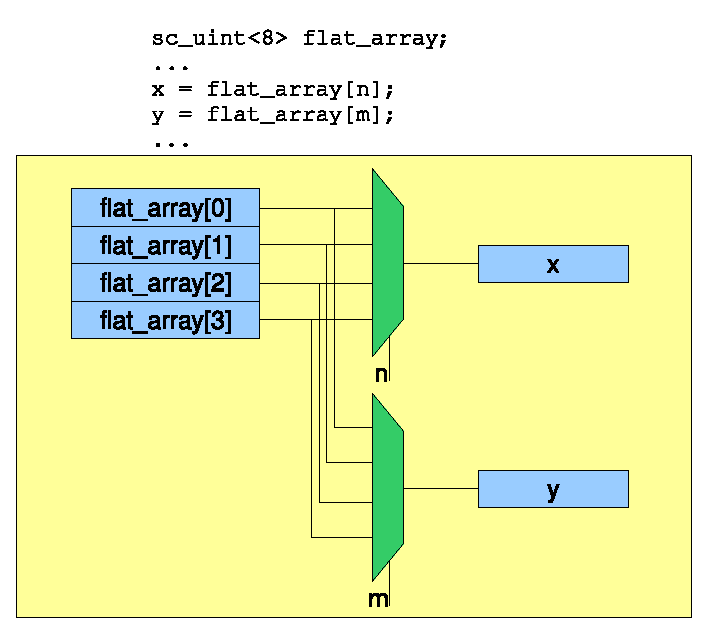
\includegraphics{figs/flatten.eps}
\caption{Improper access to flattened arrays}
\label{fig:flatten}
\end{figure}

Another point worth noticing is about design partitioning. The proper partitioning of modules and threads allows optimizations to be tested easier and speed up the synthesis of the design, allowing more time for testing different RTL implementations of the behavioral design. Another advantage of partitioning is that the design will be much easier to debug and later on the synthesis flow it will allow focusing only on problematic modules.

Finally the last and most complicated problem is unexpected simmulation mismatches between the behavioral model and RTL C++ code. Many bugs were found on the synthesis tool in this way. This shows that the tool is still in the bleeding edge of the technology and if pushed too hard sometimes it fails to generate a correct RTL implementation. There is no systematic way of working with this kind of problem. The usual approach is try to rewrite the behavior using other constructs and notifying the vendor of the problem. The VLC module has stumbled upon several of this kind of problems and the way to work around the problems was to schedule the operations manually by inserting SystemC wait() statements between operations.

\subsubsection{Placement and Routing and Timing Closure}

On the final step before prototyping some issued arose that made both back-annotated functional simulation and timing analysis to fail.

The first point that caused the failure in most modules was the aggressiveness of Cynthesizers' decisions when scheduling the operations. The vendor explains that Cynthesizer is optimistic when scheduling the datapaths because it considers that optimizations from logic synthesis will allow the design do pass timing checks. For the case of this design this was not true. The problem was easily solved by adjusting a cycle slack to the behavioral synthesis tool. A cycle slack is a period that the user pass to the tool that tells the tool to run synthesis for the clock period minus the slack period.
After adjusting the cycle slack several modules passed.

Another reason that caused simulations to fail is that the behavioral synthesis tool is not aware from the delays inserted by input and output pin logic from the FPGA. It considers that data is immediately available on the pins, which is not true, IO pins tend to be the slowest components in an FPGA. Do circumvent this issue there is the need to specify an input and output delay, calculated based on the FPGA technology, to be applied in logic synthesis. This is easely specifyed in an SDC (synopsys design constraint) script that is passed to logic synthesis.

\subsection{Prototyping Platform}

To test the design a platform was build inside the FPGA to allow data to be sent to an external device. The NiosII soft-core from Altera was used as the processor. NiosII uses the Avalon \cite{avalon} bus to communicate with the devices, so an Avalon Slave interface was implemented on the encoder. Figure \ref{fig:platform} shows the prototyping platform implemented inside the FPGA as a System on Chip (SoC).

This platform uses only a subset of the whole encoder and is capable of only encoding I-type frames. This limitation was chosen due to complexity of interfacing the Reference module with an external DDR memory that is present on the development board used to test this prototype.

\begin{figure}[h]
\centering
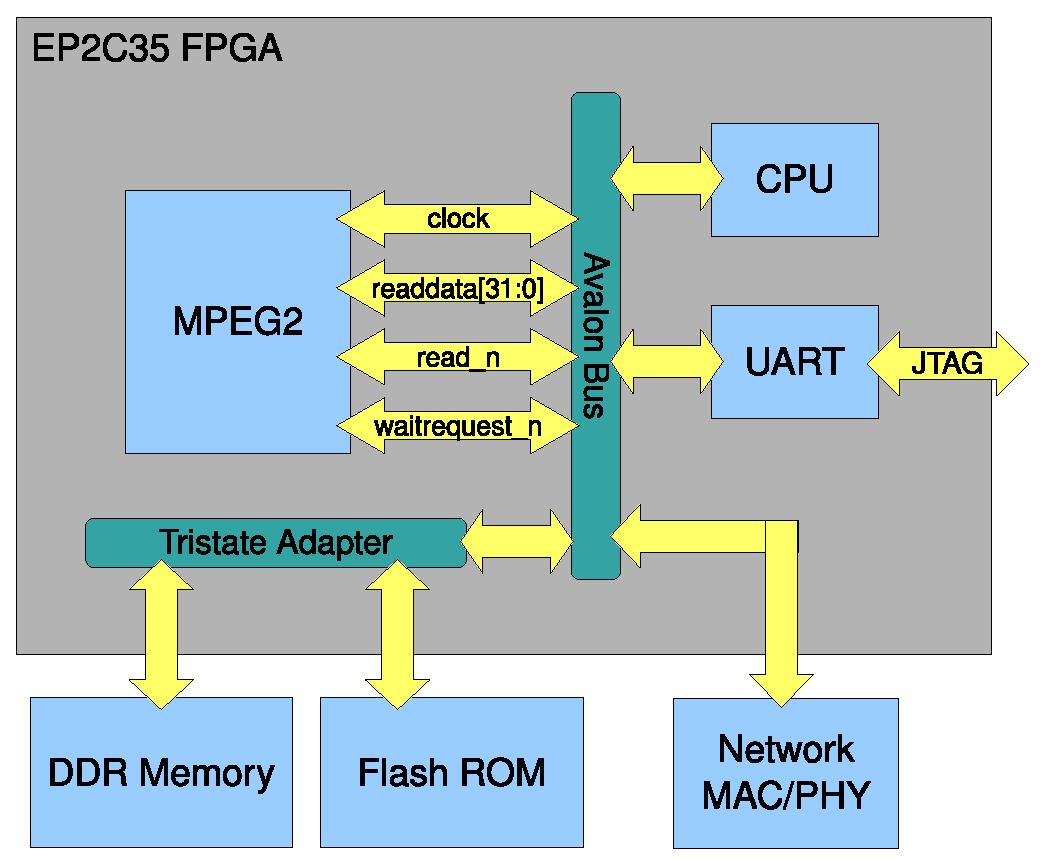
\includegraphics[width=13cm]{figs/platform.eps}
\caption{Prototyping platform}
\label{fig:platform}
\end{figure}

$\mu$CLinux \cite{uclinux}, a stripped down version of the Linux kernel, designed to run on CPUs without a memory management unit, was chosen as the operating system because of out-of-the-box support for networking. This setup allows easy streaming of the coded bit-stream to an external device, in this case a PC was used.


\subsection{Results}

As an outcome from the effort on this work several results were obtained. This section will first talk about the synthesis configurations that were experimented and how each module is affected by them, following that the synthesis results are presented and finally the subset used for prototipation is explained.

\begin{table}[h]
\centering
\begin{tabular}{|l||c|c|c|c|c|c|}
\hline
  & \multicolumn{6}{|c|}{Synthesis Configurations} \\ \hline
  		& BASIC & PIPE  & MID   	& FST1  		& FST2  		& ASAP  \\ \hline
FrameControl 	&	& X	& X		& A$^*$  		& X			& S 	\\ \hline
DCT 		&       & X     & D$^*$	 	& U$^*$ F$^*$ D$^*$  	& D$^*$ U$^*$ F$^*$ P9  & S     \\ \hline
Quantizer	&       & X     & D$^*$	 	& U$^*$ F$^*$    	& D$^*$ U$^*$ F$^*$ 	& S     \\ \hline
VLC 		&       & P9    & X     	& U$^*$ F$^*$    	& D$^*$ U$^*$ F$^*$ A   $^*$& S P9   \\ \hline
Stream 		&       & X     & X		& A$^*$ $^D*$		& X			& S     \\ \hline
Match 		&       & X     & X      	& P9 A$^*$ D$^*$	& X			& S     \\ \hline
IQuantizer 	&       & P9    & D$^*$		& U$^*$ F$^*$    	& D$^*$ U$^*$ F$^*$  	& S     \\ \hline
IDCT 		&       & P9    & D$^*$		& U$^*$ F$^*$   	& D$^*$ U$^*$ F$^*$     & S     \\ \hline
IMotion 	&       & X     & D$^*$		& A$^*$ D$^*$ U		& X		        & S     \\ \hline
MV Coder 	&       & X     & X	 	& A$^*$ D$^*$ 		& X			& S     \\ \hline
Reference 	&       & X     & X     	& X      		& X      		& S     \\ \hline

\end{tabular}
\caption{Synthesis configurations used and it's options}
\label{tab:synthconfigs}
\end{table}

As explained earlier one of the great strengths of behavioral synthesis is the opportunity to explore the design space very quickly, without having to redesign the system architecture. In the MPEG encoder presented in this text different RTL implementation options have been generated for each module. 
This allows the best option to be picked according to the desired application requirements. Table \ref{tab:synthconfigs} enlists all the synthesis configurations used and what optimizations or transformations are applied to each module. The letters and symbols in the table body mean the following:
\begin{itemize}
\item U: loop unrolling is applied;
\item A: aggressive scheduling is applied;
\item F: array flattening is applied;
\item P\#: pipelining is applied with initiation interval \#;
\item L: latency from input to output is constraned a maximum amount of clock cycles;
\item D: data path optimization is applied;
\item S: all operations are scheduled as soon as possible and all global optimizations are on;
\item X: configurations marked with an X are not used on the corresponding module;
\item * modifier: the directive is applied globally on module.
\end{itemize}

After selecting the directives for each synthesis configuration each module was synthesized and simulated to check if the generated RTL worked. The synthesis results are presented in table \ref{tab:synthres}. The numbers in the data column labled with LE represents the number of logic elements used from the target FPGA, which in total contanis about 35000 logic elements, the number in parenthesis being the amount used for multiplexing. Next to it the column labled REG represents the count of register bits used by the module for that specific synthesis configuration and the LAT column representing the latency cycles (worst case) for each data block processed by the module (without accounting pipelining). Synthsis configurations that were not used in the modules are left in blank.

\begin{landscape}
\begin{table}[h]
\centering
\begin{tabular}{|l||c|c|c |c|c|c |c|c|c |c|c|c |c|c|c |c|c|c |}
\hline
 & \multicolumn{3}{|c|}{BASIC} &
   \multicolumn{3}{|c|}{PIPE} &
   \multicolumn{3}{|c|}{MID} &
   \multicolumn{3}{|c|}{FST1} &
   \multicolumn{3}{|c|}{FST2} &
   \multicolumn{3}{|c|}{ASAP} \\ \hline
%
 		& LUT  & REG & LAT & LUT  & REG & LAT & LUT  & REG & LAT & LUT  & REG & LAT & LUT  & REG & LAT & LUT  & REG & LAT \\ \hline
Frame		&1008 &979&2794k &  -   &  -  &  -  &  -   &  -  &  -  &1325  &763&1965k&   -  &  -  & -   &1608  &1862 &3209k\\ \hline
DCT		&1292  &1562 &1795 &13214 &8806 &33   &2070  &1322 &1795 &3849  &3348 &157  &12828 &7641 &38   &16998 &4963 &22   \\ \hline
Quant.		&1774  &935  &755  &  -   &  -  &  -  &1713  &931  &755  &2939  &2112 &83   &5927  &2399 &85   &7155  &3539 &40   \\ \hline
VLC		&3773  &5751 &844  &10051 &6753 &844  &  -   &  -  & -   &3210  &5743 &844  &3314  &2466 &845  &13412 &6899 &844  \\ \hline
Stream		&574   &198  &4    &  -   &  -  &  -  &  -   &  -  & -   &726   &305  &5    &  -   &  -  & -   &828   &232  &3    \\ \hline
Match		&3099  &2089 &6003 &  -   &  -  &  -  &  -   &  -  & -   &2674  &2358 &8817 &  -   &  -  & -   &4905  &3370 &6129 \\ \hline
IQuant.		&826   &477  &553  &  -   &  -  &  -  &528   &791  &553  &2774  &3333 &27   &2774  &3333 &27   &2848  &4334 &26   \\ \hline
IDCT		&1201  &1463 &2275 &  -   &  -  &  -  &2967  &1835 &247  &6222  &5738 &111  &6222  &5738 &111  &12373 &6664 &34   \\ \hline
IMotion		&1831  &607  &3980 &  -   &  -  &  -  &1311  &632  &2822 &1620  &1219 &5174 &  -   &  -  & -   &2871  &1048 &2054 \\ \hline
MV Code	 	&822   &305  &8    &  -   &  -  &  -  &  -   &  -  & -   &820   &477  &10   &  -   &  -  & -   &1523  &359  &5    \\ \hline
Refer.		&654   &470  &46   &  -   &  -  &  -  &  -   &  -  & -   &  -   &  -  &  -  &  -   &  -  & -   &895   &377  &39   \\ \hline
\end{tabular}
\caption{Resource usage for each module}
\label{tab:synthres}
\end{table}
\end{landscape}

After the synthesis of each module some simulations must be run to see which combination of configurations provide better performance so it can be picked to go through logic synthesis and placement and routing. Table \ref{tab:combination} shows the combibations of synthesis configurations that were pickes for the benchmarking while table \ref{tab:fps} shows the resulting frame rate for each of those combinations, remembering that 24 frames per second is the desired rate. For these tests only the modules used for the prototype (which generates only I-type frames) were used.

\begin{table}[h]
\centering
\begin{tabular}{|l||c|c|c|c|c|c|}
\hline
		& CFG1	& CFG2	& CFG3	& CFG4	& CFG5 & CFG6 \\ \hline
FrameControl 	& BASIC	& BASIC	& BASIC & FST1  & FST1 & ASAP \\ \hline
DCT		& BASIC & MID   & FST1  & FST1  & FST2 & ASAP \\ \hline
Quantizer	& BASIC & MID   & FST1  & FST1  & FST2 & ASAP \\ \hline
VLC		& BASIC & BASIC & FST1  & PIPE  & PIPE & ASAP \\ \hline
Stream		& BASIC & BASIC & BASIC & FST1  & FST1 & ASAP \\ \hline
\end{tabular}
\caption{Selected combinations of synthesis configurations}
\label{tab:combination}
\end{table}

\begin{table}[h]
\centering
\begin{tabular}{|l|c|c|}
\hline
Combination & Frame Rate & Total Area (LUT) \\ \hline
CFG1 & 1.1 & 8361\\ \hline
CFG2 & 2 & 9138\\ \hline
CFG3 & 7 & 11580\\ \hline
CFG4 & 26  & 18890 \\ \hline
CFG5 & 30  & 30917\\ \hline
CFG6 & 49  & 30001 \\ \hline
\end{tabular}
\caption{Framerate obtained for each combination of synthesis configurations }
\label{tab:fps}
\end{table}

With information from table \ref{tab:fps} it's possible to pick the design that fits the requirements using the minimum area. It's also possible to plot a graph that shows the results mapped into the design space, which is shown in figure \ref{fig:designspace}. The analysis of this data leads to pick the combinantion named CFG4 as the option to be prototyped beacause it's the configuration that beats 24fps taking the minimum area among the others. With further design space exploration and some fine-tuning it should to be possible to reduce area to less than 15000 LUTs while still beating 24fps performance.

\begin{figure}[h]
\centering
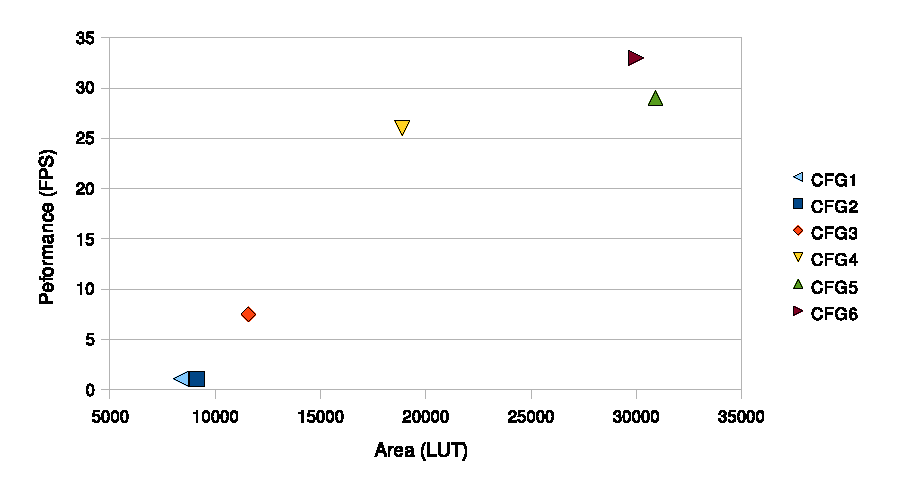
\includegraphics{figs/designspace.eps}
\caption{Graph of the explored design space}
\label{fig:designspace}
\end{figure}



\subsection{Future Works}

There are several points in this effort that may offspring other works. First of it is improving the encoder. A first improvement would be to finish off the DDR memory interface implementation on the Reference module to allow the prototipation of a system that encodes P-type frames. Another improvement would be a rate control module that would adapt the quantization factor in order to mantain the output bit rate constant, an initial study was done in this direction but it was not implemented as of the writing of this text. Figure \ref{fig:ratecontrol} shows a possible architecture for this module.

\begin{figure}[h]
\centering
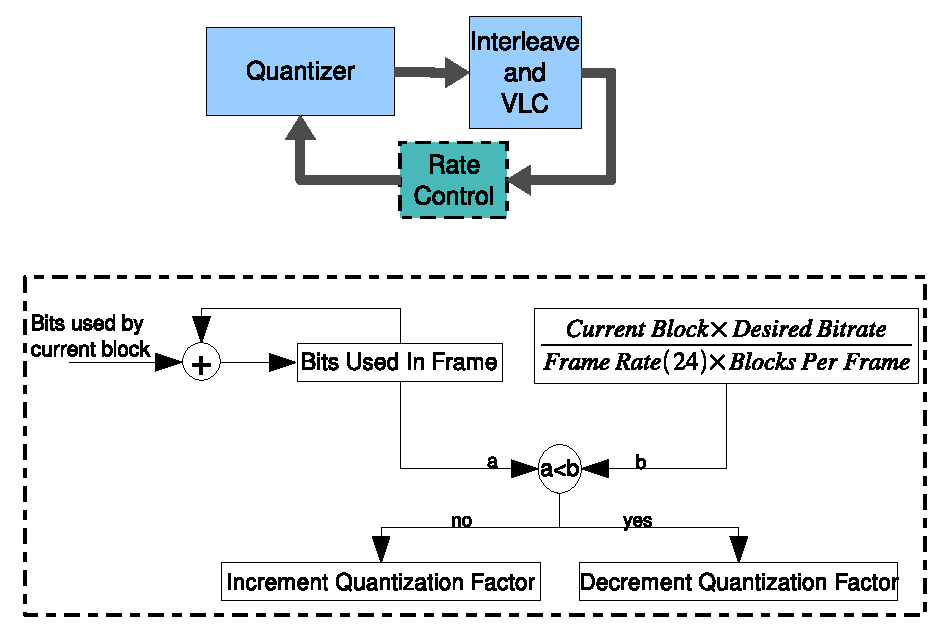
\includegraphics{figs/ratecontrol.eps}
\caption{Suggested architecture for a rate control module}
\label{fig:ratecontrol}
\end{figure}

Another point that still needs work is the motion estimator (Match module) in which the architecture was not fully explored. An interesting change in the architecture would be adding burst transfers instead of the current method in which for each pixel transfered from the Reference module one request is needed, adding significant overhead.
Also other algorithms could be studied to replace the simple three step search implemented for motion compensation. Using phase correlation may even be feasible since transformations to the frequency domain can be very efficient in hardware, as some recent works \cite{motion_phase_hw} shows this.

In the sense of behavioral synthesis a better and careful study of the code aspects that tend cause simulations mismatches can be done. One starting point would be deeply studing the Interleave and VLC module (since it was quite problematic) and learning how each operation is scheduled. This can be quite useful for other works that rely on behavioral synthesis and also for the software vendors to improve the quality of their tools.

\pagebreak

\section*{Conclusion}
\phantomsection
\addcontentsline{toc}{section}{Conclusion}

With the closing of this work it possible to conclude that behavioral synthesis eases and speeds up the design and implementation steps of a system, since it can take a high level description and generate several different RTL architectures. The MPEG encoder developed in this work took much less effort than the decoder cited in \cite{brazilip} which was developed using RT-level synthesis. Another important advantage is that the different architectures that were generated may suite different needs, for example embedded use on consumer electronics versus real-time encoding for transmission.

This work also contributes to the understanding the source of some difficulties that may arise from the use of a behavioral synthesis tool, since it's a technology that is still in a maturing stage and does not have the two-decade expertise that the RTL synthesis community has gathered.

Relevant knowlege was also obtained in the analysis of digital processing and compression algorithms and the gains that behavioral synthesis can achieve in each of those algorithms, for example it's possible to see in the results section that the DCT designs space is quite large, the area ranges from 2000 logic elements in the most simple configuration to 17000 elements in the most performance-optimized version, in the opposite side of that is the VLC coder in which all the synthesis configurations the area was close to 3500 logic elements with little impact on latency.

Also as this is a large work there were some issues that were left open in the decoder that may be concluded in the future by a descendent effort.

\pagebreak
\bibliographystyle{unsrt}
\phantomsection
\addcontentsline{toc}{section}{Bibliography}
\bibliography{myrefs}


\pagebreak
\section*{CD-ROM}
\addcontentsline{toc}{section}{CD-ROM}
This CD-ROM contains the source code of the design presented in this work. A digital copy of this document is also enclosed in Adobe PDF and PostScript formats.
\end{document}
